They key insights for this comes from the \textbf{PPAD}-inclusion proof
by Deligkas et al. \cite{deligkas_PureCircuitTightInapproximability_2024}, where they
showed that we can reduce PureCircuit, to \textit{Brouwer} problem by constructing
a continuous function $F: [0,1]^n \to [0,1]^n$ as such: For each $v \in V$, we create
continuous functions $f_i(\cdot): [0,1]^n \to [0,1]$ where we take the input of vector
of all the nodes and output the value of the current node
\begin{enumerate}
    \item If $v \in V$ is the output of a $\textsc{NOR}$ gate with inputs $x_1, x_2$, then we have:
          $$
              f_v(\mathbf{x}) := (1 - \mathbf{x}_{x_1}) \cdot (1 - \mathbf{x}_{x_2})
          $$
    \item If $y_1, y_2$ are the outputs of a  $\textsc{Purify}$ gate with $z$ as input, then we have:
          \begin{align*}
              f_{y_1}(\mathbf{x}) & := \max\{2 \cdot \mathbf{x}_{z} - 1, 0\} \\
              f_{y_2}(\mathbf{x}) & := \min\{2 \cdot \mathbf{x}_{z}, 1\}
          \end{align*}
\end{enumerate}
If $F(x) = x$, then we also found a solution for \textit{PureCircuit} by:
$$
    \forall v \in V: \mathbf{x}[v] = \begin{cases}
        0    & \mathbf{x}[v] = 0     \\
        \bot & 0 < \mathbf{x}[v] < 1 \\
        1    & \mathbf{x}[v] = 1     \\
    \end{cases}
$$
We assume that the \textit{Purify} gate is satisfied for any pair outputs
as long as the output is not $(\bot, \bot)$. Using that we can define two types of variants
of \textit{PureCircuit} that are parsimoniously reducible to \textit{SourceOrPresink}.
We first define \textit{SourceOrPresink} as:

\begin{definitionbox}{$\textit{SourceOrPresink}$ definition \cite{ikenmeyer_WhatWhatNot_2022}}{source-or-presink-def}
    \label{def:source-or-presink-def}
    A $\textit{SourceOrPresink}$ is defined by the same construction as the $\textit{EndOfLine}$
    but the solutions are sources and predecessors of sinks. If a node is both a source
    and a presink, then we count it once.
\end{definitionbox}

We will annotate our \textit{Purify} gates with an additional bit $b \in \mathbb{B}$ such that
$$
    \forall x \in \mathbb{T}, y_1, y_2 \in \mathbb{T}: \textsc{Purify}^b(x) = (y_1,y_2) \implies \textsc{Purify}^{\neg {b}}(x) = (y_2, y_1)
$$
We can create two types of problems based on the annotation:
\begin{enumerate}
    \item \textit{AcyclicPureCircuit}: Our instance is acyclic
    \item \textit{Permutation-freePC}: Each \textsc{Purify} gate must have its outputs connected to a permutation-free
          circuit $C$ such that:
          $$
              \forall x \in \mathbb{T}^n, \sigma \in \mathcal{A}: C(\sigma(x)) = C(x)
          $$
          Where $\mathcal{A}$ is the set of automorphisms of $[n] \to [n]$.
\end{enumerate}

We now demonstrate how we can pair two solutions of each of the problems above:
\paragraph*{AcyclicPureCircuit} Assume we have a satisfying assignment $\mathbb{x}$.
For each \textsc{Purify} pair, we can flip the outputs such that in our new assignment $\mathbb{x'}$,
$\forall (\textsc{Purify}, \cdot, a,b) \in G:, \mathbb{x'}[b] =\mathbb{x}[a] \wedge \mathbb{x'}[a]  = \mathbb{x}[b]$



\begin{figure}[h!]
    \centering


    \tikzset{every picture/.style={line width=0.75pt}} %set default line width to 0.75pt        

    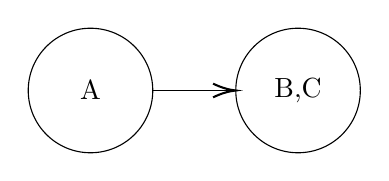
\begin{tikzpicture}[x=0.75pt,y=0.75pt,yscale=-1,xscale=1]
        %uncomment if require: \path (0,260); %set diagram left start at 0, and has height of 260

        %Shape: Circle [id:dp7760056968770814] 
        \draw   (90,140) .. controls (90,123.43) and (103.43,110) .. (120,110) .. controls (136.57,110) and (150,123.43) .. (150,140) .. controls (150,156.57) and (136.57,170) .. (120,170) .. controls (103.43,170) and (90,156.57) .. (90,140) -- cycle ;

        %Shape: Circle [id:dp22383258291194785] 
        \draw   (190,140) .. controls (190,123.43) and (203.43,110) .. (220,110) .. controls (236.57,110) and (250,123.43) .. (250,140) .. controls (250,156.57) and (236.57,170) .. (220,170) .. controls (203.43,170) and (190,156.57) .. (190,140) -- cycle ;

        %Straight Lines [id:da1444295916995948] 
        \draw    (150,140) -- (188,140) ;
        \draw [shift={(190,140)}, rotate = 180] [color={rgb, 255:red, 0; green, 0; blue, 0 }  ][line width=0.75]    (10.93,-3.29) .. controls (6.95,-1.4) and (3.31,-0.3) .. (0,0) .. controls (3.31,0.3) and (6.95,1.4) .. (10.93,3.29)   ;

        % Text Node
        \draw (120,140) node   [align=left] {A};
        % Text Node
        \draw (220,140) node   [align=left] {B,C};


    \end{tikzpicture}
    \caption{Equal solution conversion}
    \label{fig:equal}
\end{figure}
Otherwise for two distinct solutions we can use the following
\begin{figure}[h!]
    \centering
    \tikzset{every picture/.style={line width=0.75pt}} %set default line width to 0.75pt
    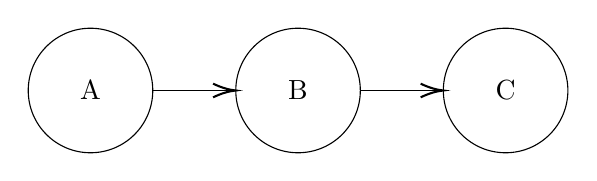
\begin{tikzpicture}[x=0.75pt,y=0.75pt,yscale=-1,xscale=1]
        %uncomment if require: \path (0,260); %set diagram left start at 0, and has height of 260

        %Shape: Circle [id:dp7760056968770814] 
        \draw   (90,140) .. controls (90,123.43) and (103.43,110) .. (120,110) .. controls (136.57,110) and (150,123.43) .. (150,140) .. controls (150,156.57) and (136.57,170) .. (120,170) .. controls (103.43,170) and (90,156.57) .. (90,140) -- cycle ;

        %Shape: Circle [id:dp22383258291194785] 
        \draw   (190,140) .. controls (190,123.43) and (203.43,110) .. (220,110) .. controls (236.57,110) and (250,123.43) .. (250,140) .. controls (250,156.57) and (236.57,170) .. (220,170) .. controls (203.43,170) and (190,156.57) .. (190,140) -- cycle ;

        %Shape: Circle [id:dp48038379742035975] 
        \draw   (290,140) .. controls (290,123.43) and (303.43,110) .. (320,110) .. controls (336.57,110) and (350,123.43) .. (350,140) .. controls (350,156.57) and (336.57,170) .. (320,170) .. controls (303.43,170) and (290,156.57) .. (290,140) -- cycle ;

        %Straight Lines [id:da1444295916995948] 
        \draw    (150,140) -- (188,140) ;
        \draw [shift={(190,140)}, rotate = 180] [color={rgb, 255:red, 0; green, 0; blue, 0 }  ][line width=0.75]    (10.93,-3.29) .. controls (6.95,-1.4) and (3.31,-0.3) .. (0,0) .. controls (3.31,0.3) and (6.95,1.4) .. (10.93,3.29)   ;
        %Straight Lines [id:da6754989440526618] 
        \draw    (250,140) -- (288,140) ;
        \draw [shift={(290,140)}, rotate = 180] [color={rgb, 255:red, 0; green, 0; blue, 0 }  ][line width=0.75]    (10.93,-3.29) .. controls (6.95,-1.4) and (3.31,-0.3) .. (0,0) .. controls (3.31,0.3) and (6.95,1.4) .. (10.93,3.29)   ;

        % Text Node
        \draw (120,140) node   [align=left] {A};
        % Text Node
        \draw (220,140) node   [align=left] {B};
        % Text Node
        \draw (320,140) node   [align=left] {C};
    \end{tikzpicture}
    \caption{Not equal solution}
    \label{fig:not-equal}
\end{figure}


